\documentclass[a4paper]{report}
\linespread{1.5} % ajouter un espacement entre les lignes de tout le document 
%====================== PACKAGES ======================
%\documentclass{article}
\usepackage{xcolor}
\usepackage{listings}
\definecolor{mGreen}{rgb}{0,0.6,0}
\definecolor{mGray}{rgb}{0.5,0.5,0.5}
\definecolor{mPurple}{rgb}{0.58,0,0.82}
\definecolor{backgroundColour}{rgb}{0.95,0.95,0.92}

\lstdefinestyle{CStyle}{
    backgroundcolor=\color{backgroundColour},   
    commentstyle=\color{mGreen},
    keywordstyle=\color{magenta},
    numberstyle=\tiny\color{mGray},
    stringstyle=\color{mPurple},
    basicstyle=\footnotesize,
    breakatwhitespace=false,         
    breaklines=true,                 
    captionpos=b,                    
    keepspaces=true,                 
    numbers=left,                    
    numbersep=5pt,                  
    showspaces=false,                
    showstringspaces=false,
    showtabs=false,                  
    tabsize=2,
    language=java
}






\usepackage{multirow}
\usepackage{algorithm}
\usepackage{algorithmic}
\usepackage[french]{babel}
\usepackage[utf8x]{inputenc}
%pour gérer les positionnement d'images
\usepackage{float}
\usepackage{amsmath}
\usepackage{graphicx}
\usepackage[colorinlistoftodos]{todonotes}
\usepackage{url}
%pour les informations sur un document compilé en PDF et les liens externes / internes
\usepackage{hyperref}
%pour la mise en page des tableaux
\usepackage{array}
\usepackage{tabularx}
%pour utiliser \floatbarrier
%\usepackage{placeins}
%\usepackage{floatrow}
%espacement entre les lignes
\usepackage{setspace}
%modifier la mise en page de l'abstract
\usepackage{abstract}
%police et mise en page (marges) du document
\usepackage[T1]{fontenc}
\usepackage[top=2cm, bottom=2cm, left=2cm, right=2cm]{geometry}
%Pour les galerie d'images
\usepackage{subfig}

\usepackage{longtable}
\usepackage{svg}
\svgpath{{../imgs/}}

%============= INFORMATION ET REGLES =============

%rajouter les numérotation pour les \paragraphe et \subparagraphe
\setcounter{secnumdepth}{4}
\setcounter{tocdepth}{4}

\hypersetup{							% Information sur le document
pdfauthor = {EL MRABTI Hamza},			% Auteurs
pdftitle = {Système de santé},			% Titre du document
pdfsubject = {Système de santé},		% Sujet
pdfkeywords = {Tag1, Tag2, Tag3, ...},	% Mots-clefs
pdfstartview={FitH}}					% ajuste la page à la largueur de l'écran
%pdfcreator = {MikTeX},% Logiciel qui a crée le document
%pdfproducer = {}} % Société avec produit le logiciel

%======================== DEBUT DU DOCUMENT ========================

\begin{document}

%régler l'espacement entre les lignes
\newcommand{\HRule}{\rule{\linewidth}{0.5mm}}

%page de garde
\begin{titlepage}
\begin{center}

% Upper part of the page. The '~' is needed because only works if a paragraph has started.

\includegraphics[width=1\textwidth]{./ensiass}~\\[1.5cm]

\textsc{\Large Ecole Nationale Supérieure d’Informatique et d’Analyse des Systèmes - RABAT }\\[2cm]

\textsc{\Large Rapport de Stage de Première Année
}\\[0.5cm]

% Title
\HRule \\[0.4cm]

{\huge \bfseries   
 Gestion des données d'un patient dans un système de santé muti-centres
 \\[0.4cm] }
\HRule \\
[2cm]
% Author and supervisor
\begin{minipage}{0.4\textwidth}
\begin{flushleft} \large
\emph{Réalisé par :}\\
Hamza \textsc{El Mrabti}\\ [1cm]

\emph{Filière :} \\
\textsc{Génie Logiciel }\\



\end{flushleft}
\end{minipage}
\begin{minipage}{0.4\textwidth}
\begin{flushright} \large
\emph{Encadré par:} \\
Dr. Reda \textsc{Ahroum}\\[1cm]
\emph{Memebres du jury:} \\
Pr. xxxxxxx \textsc{yyyyy}\\
Pr. wwww \textsc{zzzzzzz}\\[1cm]


\end{flushright}
\end{minipage}

\vfill

% Bottom of the page
{\large \ Année Scolaire 2022/2023}

\end{center}
\end{titlepage}

%page blanche 
\newpage
~
%ne pas numéroter cette page
\thispagestyle{empty}
%\newpage  ==> pour créer une nouvelle page

%\thispagestyle{empty}
\chapter*{Dédicaces}

\vspace*{\stretch{0.5}}
\begin{flushright}
\emph{\`A ma famille, à mes amis, à tous ceux qui me sont chèrs } \\
\textsc{Hamza El Mrabti}\\
\end{flushright}

\vspace*{\stretch{0.2}}


\vspace*{\stretch{1}}




\thispagestyle{empty}

\chapter*{Remerciements}



\begin{center}
``La reconnaissance est la plus belle fleur qui jaillit de l'âme "
\end{center}
\begin{center} $\sim$ Henry Beecher . \end{center}
Nous voudrions tout d'abord adresser toute notre gratitude au 
Pr. Ahmed Ettalbi, notre encadrant, pour sa patience, sa disponibilité, sa rigueur scientifique, ses qualités humaines
et surtout ses judicieux conseils, qui ont contribué à alimenter notre
réfexion.

Ensuite nous exprimons notre profonde reconnaissance aux membres du jury, notament Mme. Mounia Abik et M. Ahmed Ettalbi, pour le temps précieux qu'ils accordent volontairement en contribuant au bon déroulement du module.

Enfin nous tenons à remercier chaleureusement nos familles, nos amis et toutes les personnes qui ont contribué énormément à la réalisation de notre projet et qui nous ont aidés lors de la rédaction de ce rapport, aussi bien pour leurs encouragements et soutiens dans les moments forts.


\thispagestyle{empty}
\chapter*{Résumé}

Le présent rapport porte sur le stage de le fin de la première année du cycle d'ingénieur, filière génie logiciel à l'Ecole Supérieure d'Informatique et d'Analyse des Systèmes 

Le sujet de ce projet consistait à la migration des serious games construit par l'entreprise vers un nouveau LMS(learning management system) et puis effectuer les tests unitaire sur le LMS

 Notre travail s’est fait sur deux piliers:
 Faire la migrations des serious games vers le nouveau LMS et effectuer les tests unitaires sur tous les fonctionnalité de ce dernier.
 Grâce à l’aide de mon encadrant,  j'ai appris, durant ces derniers mois, à utiliser
différents outils et découvrir plusieurs concepts qui nous ont aidés à aboutir au objectifs demandé.
 Nous vous présenterons donc tout au long de ce rapport, les étapes que nous avons
suivis ainsi que les outils que nous avons utilisés pour réaliser notre projet. 

\textbf{Keywords} : Serious games , e-learning,  Onboarding , Migration, LMS, Tests

\thispagestyle{empty}
\chapter*{Abstract}


This report concerns the project for the end of the second year of the engineering cycle, software engineering sector at the Ecole Supérieure d'Informatique et d'Analyse des Systèmes

The subject of this project was the management of patient data in a multi-center system.

  Our work was done in several phases:
  An analysis and design phase and a development phase.
  Thanks to the help of our supervisor, we have learned, over the past few months, to use
different tools and discover several concepts that helped us to develop this application.
  We will therefore present to you throughout this report the steps we have
followed as well as the tools we used to carry out our project.

\textbf{Keywords} : Health system , Patient data ,  Medical records , e-Health 

\thispagestyle{empty}
\listoffigures
\thispagestyle{empty}
\listoftables
\thispagestyle{empty}
\tableofcontents
\thispagestyle{empty}


\setcounter{page}{0}


\chapter*{Introduction générale}



La notion de « serious game », traduite officiellement par la commission générale de
terminologie et de néologie par « jeu sérieux », peut apparaître comme un oxymore. Pourtant
depuis dix ans, il ne s'agit plus d'un simple concept ou d'un projet vague comme celui de « web
sémantique », mais bien d'une réalité suffisamment tangible pour permettre l'existence d'un vrai
marché, avec des producteurs privés et des clients, ou d'un véritable intérêt de la part de
l’Éducation Nationale. Cette dynamique est bien entendu l’un des derniers fruits de la vague
extraordinaire des jeux vidéo depuis quarante ans, ainsi que de l’émergence de la génération des
digital natives ; mais le succès du serious game est tel qu’il a bel et bien débordé largement ces
deux cadres incubateurs. Beaucoup s’y intéressent, parce qu’il est en plein essor et parce qu’il est
efficace ; mieux : il est en plein essor parce qu’il est efficace.
S'il existe plusieurs définitions du serious game, celle du spécialiste français Julian Alvarez,
pionnier de leur étude, fait autorité : « application informatique, dont l'objectif est de combiner à
la fois des aspects sérieux (Serious) tels, de manière non exhaustive, l'enseignement,
l'apprentissage, la communication, ou encore l'information, avec des ressorts ludiques issus du
jeu-vidéo (Game). Une telle association a donc pour but de s'écarter du simple divertissement. »
Il s'agit ainsi, pour simplifier à grands traits, d'un jeu vidéo, le plus souvent en ligne, utilisé à des
fins d'information ou de formation ; ou, de manière ramassée, d'une combinaison sérieuse et
vidéoludique, la seconde étant au service de la première. La vocation d’un serious game est donc
de rendre attrayante la dimension sérieuse par une forme, une interaction, des règles et
éventuellement des objectifs ludiques parmi lesquels, selon le sociologue Roger Caillois, le «goût
pour la difficulté gratuite». Le serious game intéresse potentiellement les entreprises privées, les
associations, le secteur public dont font partie les bibliothèques.
L’entreprise NowEdge, crée en 2020, propose des solutions innovantes de gamification de
l’apprentissage sous forme de serious games destinées aux entreprises et tout établissement offrant
des formations professionnelles.
Ainsi, mon présent travail s’inscrit dans le cadre du stage technique de fin de la
première année en filière GL à l'Ecole nationale supérieure d'informaitque et d'analyse des systèmes pour
l’année universitaire 2022/2023.


%ne pas numéroter le sommaire

% \newpage

%espacement entre les lignes d'un tableau
\renewcommand{\arraystretch}{1.5}

%====================== INCLUSION DES PARTIES ======================

~
%recommencer la numérotation des pages à "1"
\newpage

\chapter{Présentation du projet}

\section{Introduction}

Dans ce chapitre nous allons mettre le sujet dans son cadre général,le cahier de charge  et l’objectif de ce projet, ainsi pour obtenir une idée sur ce que va réaliser le système en termes de métier (comportement du système). Par la suite nous aborderons la méthode adoptée pour réaliser ce
projet.


\section{Problématique}


Face aux difficultés multiples que rencontre le personnel de la santé publique dans la gestion
 et l’exploitation des dossiers médicaux des patients, face aux flux de patients et compte tenu de l’importance que représente un dossier médical, l’informatisation de ce dossier présente un
enjeu stratégique majeur.
 Elle aura beaucoup de retombées sur la qualité des soins aux seins des établissements de santé d’où l’utilité et la nécessité d’un système capable de centraliser et capitaliser l’ensemble des informations générées par le patient.
 
 
\section{Description du projet}

Pour parer à ces difficultés, un système souple et sécurisé est nécessaire.
 C’est dans ce cadre que s’inscrit notre projet de fin d’année réalisé .Il s’agit d’une
Implémentation et conception d’une application web qui permet la sauvegarde, la gestion
et la manipulation des données médicaux relatives aux traitements subis par un patient.



\section{Objectifs}


L’objectif du projet est de concevoir un application web qui consiste à mémoriser
pour chaque patient, non seulement les informations administratives (âge, sexe, adresse,
contact,…), mais également des informations médicales (le diagnostic,les ordonances,
les comptes-rendus, les traitements administrés, les analyses et les résultats ,..) et tout
autre type d’actes médicaux … puisqu'il entend améliorer la saisie, la sauvegarde
et la communication des informations de santé, tout en respectant les droits du patient bien sûr , afin de garantir une gestion souple du dossier médical de ce patient.

 L’objectif sera également d’avoir une approche originale et différente par rapport au
 sujet et d’utiliser au mieux les outils dont nous disposons pour mettre au point ce projet.
La démarche que nous avons suivie pour mettre au point cette application est simple.
 Nous avons divisé notre travail en deux différentes phases:
 \begin{itemize}
 \item Une phase où nous avons analysé le sujet, décider une approche crédible pour modéliser
l’application.
 \item une phase de développement ou nous avons commencé à mettre au point l’application en créant la base de données et le site web en question.
 \end{itemize}
 

\section{Cahier de charge}

\subsection{Introduction}

Il s’agit de la conception d’un système qui gère les données des patients dans un système de santé multi-centres, il consiste à mémoriser pour chaque patient, non seulement les informations administratives (nom, âge, sexe ...), mais également des informations concernant l’historique médical du patient, ce qui aide les médecins consultés à prendre des décisions en se basant sur des données exactes et pertinentes, en offrant des interfaces personnalisées selon le profil du demandeur de l’information, et accessible à tout moment.\\
Pour cela on propose les utilisateurs suivants : 

\begin{itemize}
\item Patient
\item Médecin
\item Radiologue
\item Admin
\end{itemize}
 





\section{Conclusion}
Dans ce chapitre nous avons pu tracer le cadre générale du projet, pour préparer la surface pour l'analyse et la conception abordés dans le chapitre suivant.





\chapter{Analyse et conception}



\section{Introduction}

Ce chapitre abordera une analyse du sujet pour présenter une approche originale et une modélisation adéquate pour l’application


\subsection{Analyse du sujet}




\section{Conclusion} 

Aprés terminer cette étape d'analyse et conception nous avons une vision claire sur la réalisation qui est l'étape suivante qui vient aprés le choix des outils technologique.




\chapter{Réalisation et résultats}

\section{Introduction}

Après avoir achevé l’étape d’analyse et conception de l’application, on va entamer dans ce chapitre la partie réalisation et implémentation dans laquelle on va s’assurer que le système est prêt pour être exploité par les utilisateurs finaux. Premièrement on choisit les technologies et puis on procède à la réalisation.


\section{Outils et technologies}

tech

python



\section{Interfaces graphiques}

\subsection{Interfaces de Finedge}

\begin{center}
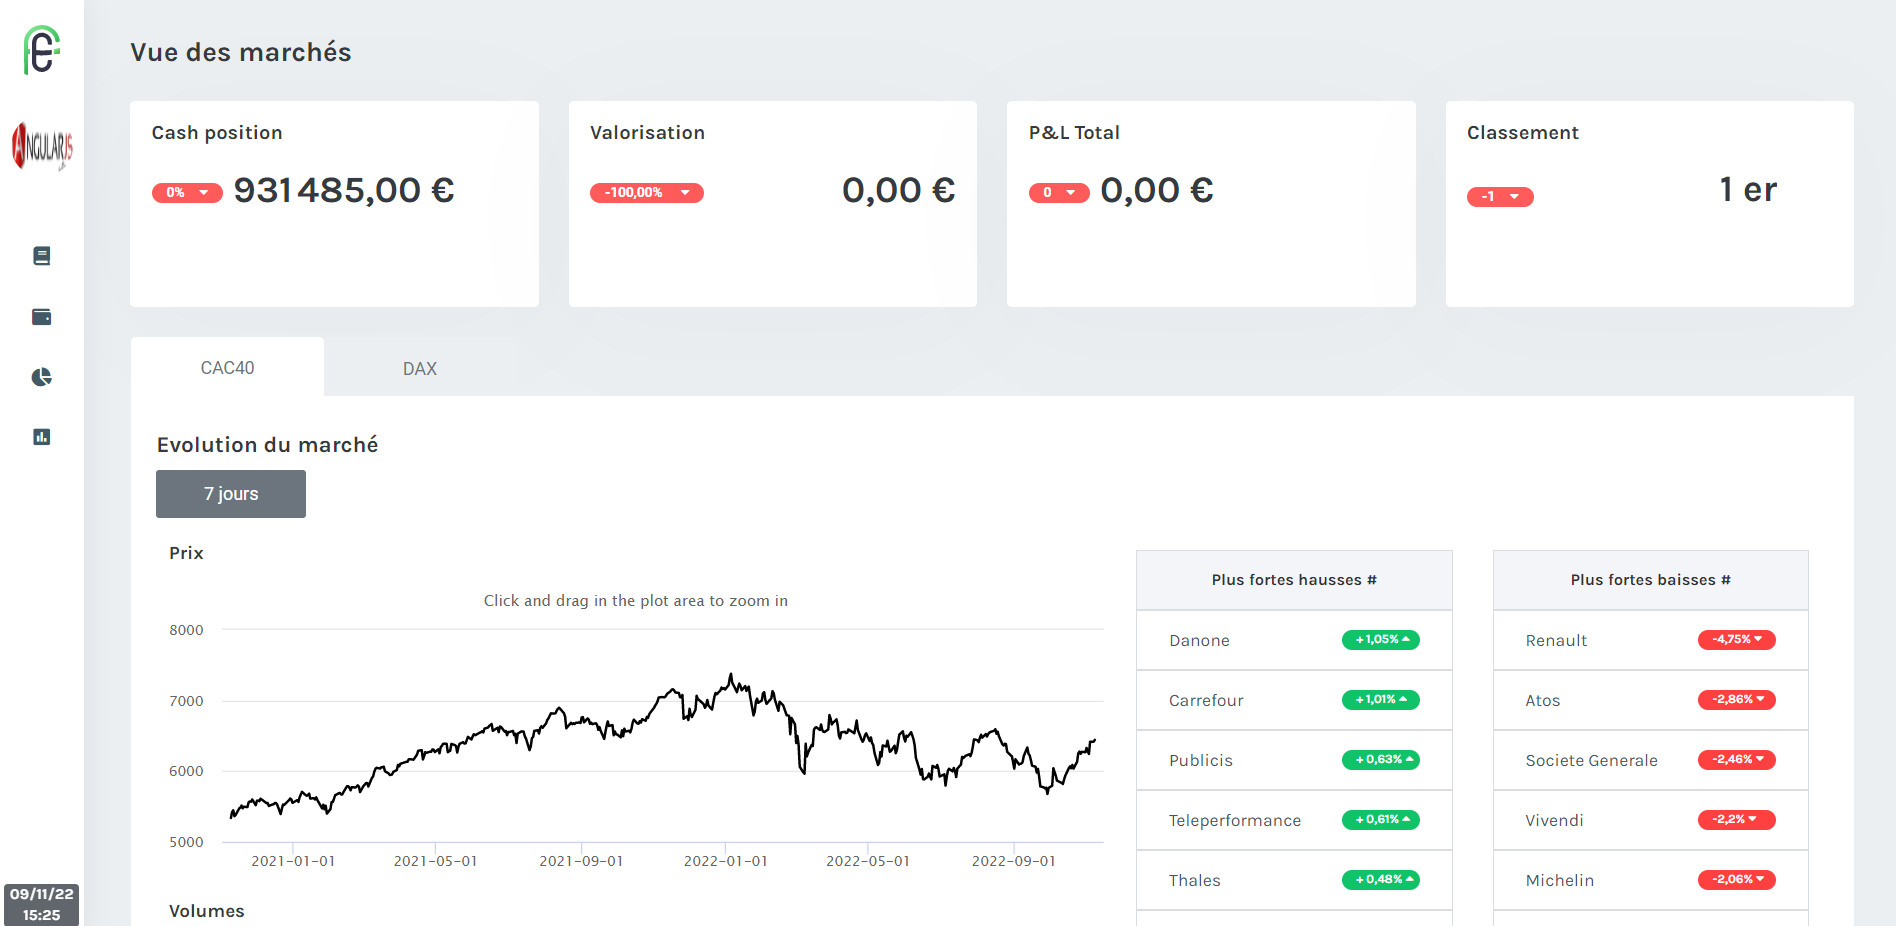
\includegraphics[scale=0.25]{images/fin} 
\end{center}


\begin{center}
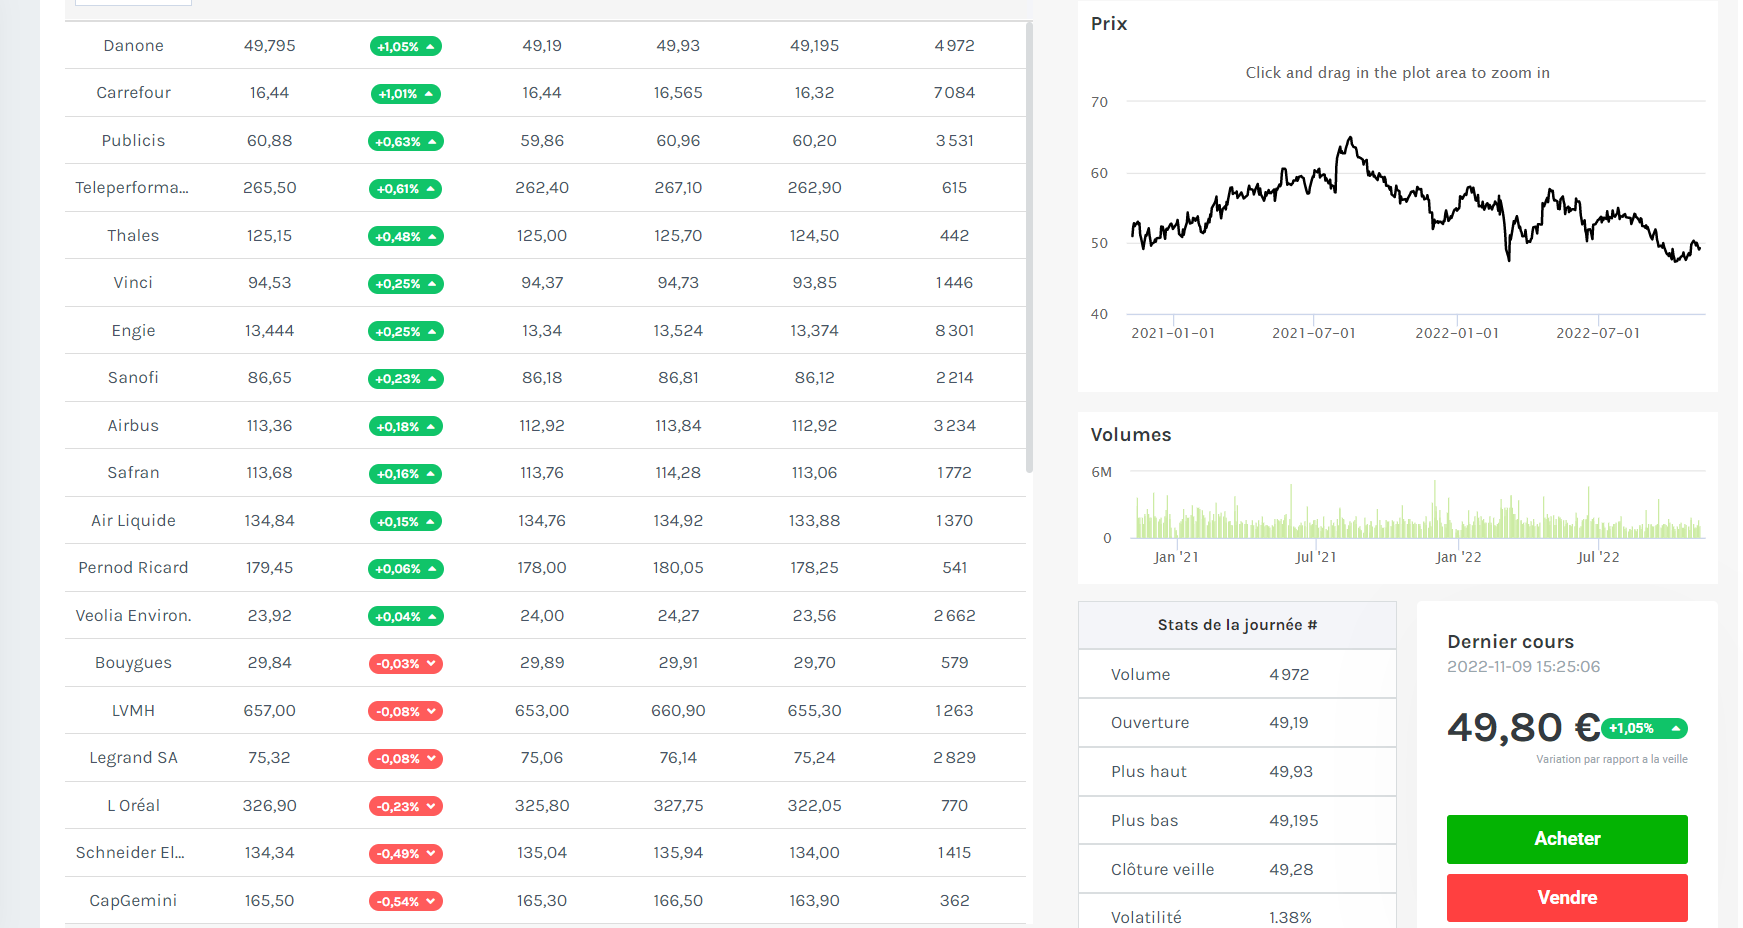
\includegraphics[scale=0.25]{images/fin2} 
\end{center}


\subsection{Interfaces de Pvgame}



\begin{center}
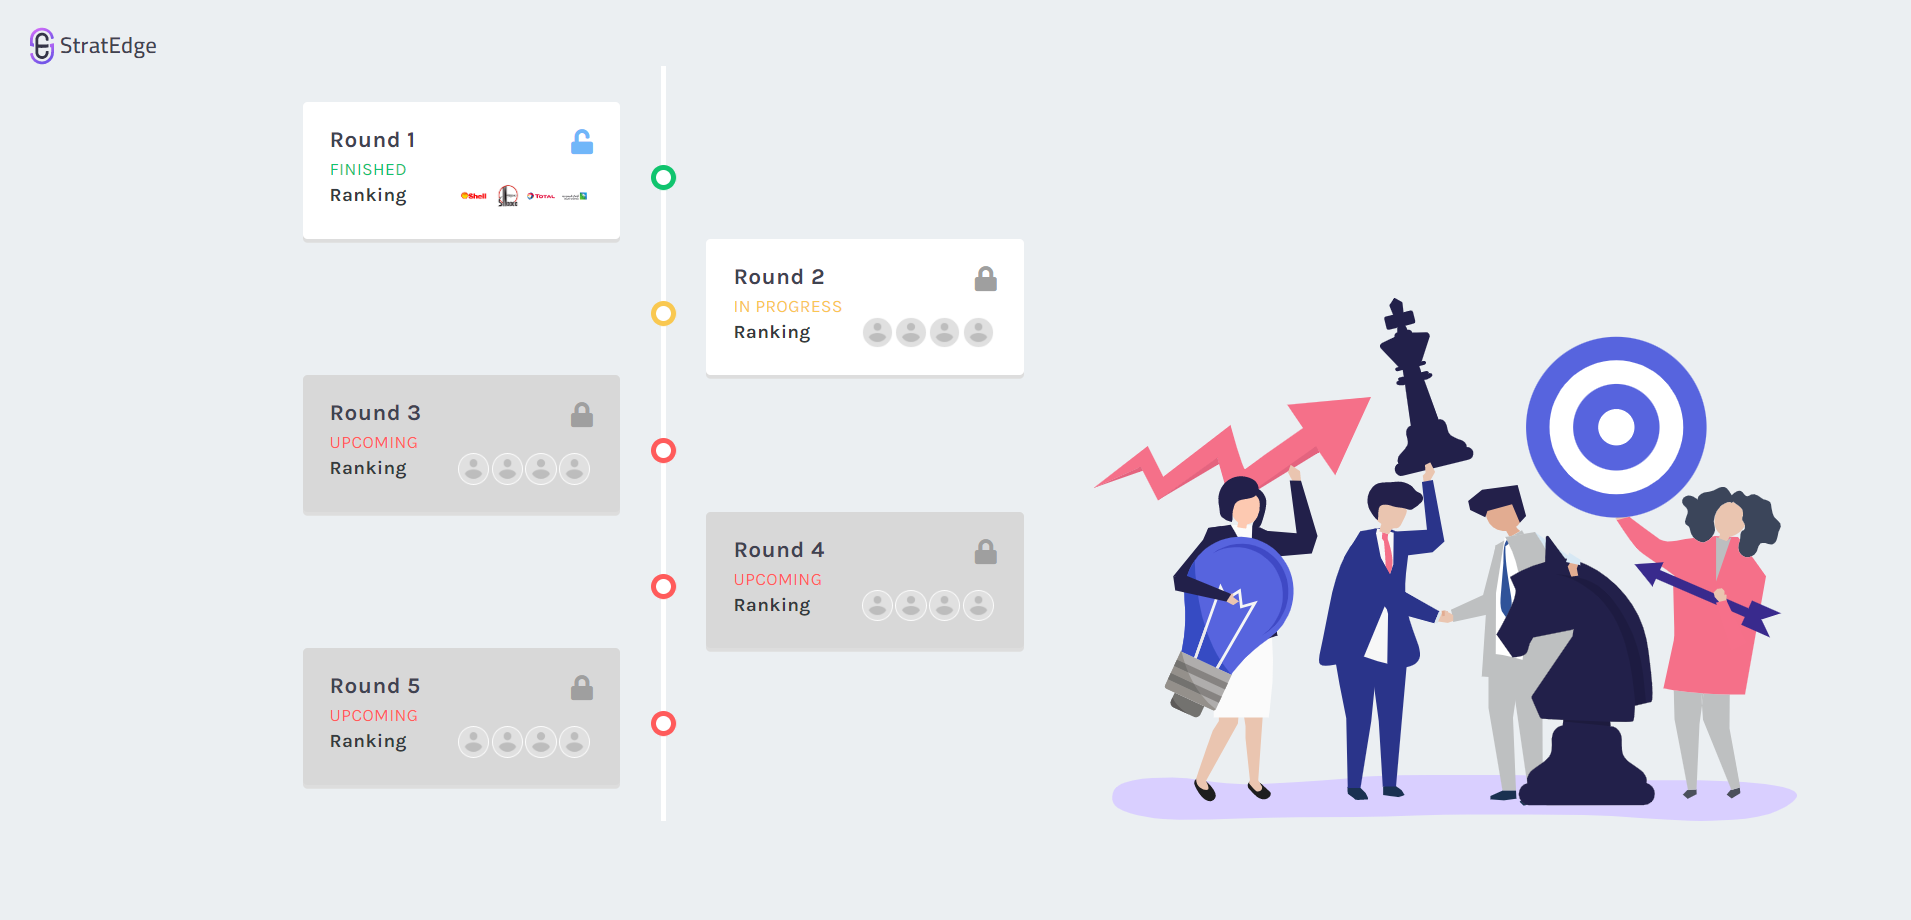
\includegraphics[scale=0.25]{images/strat} 
\end{center} 


\begin{center}
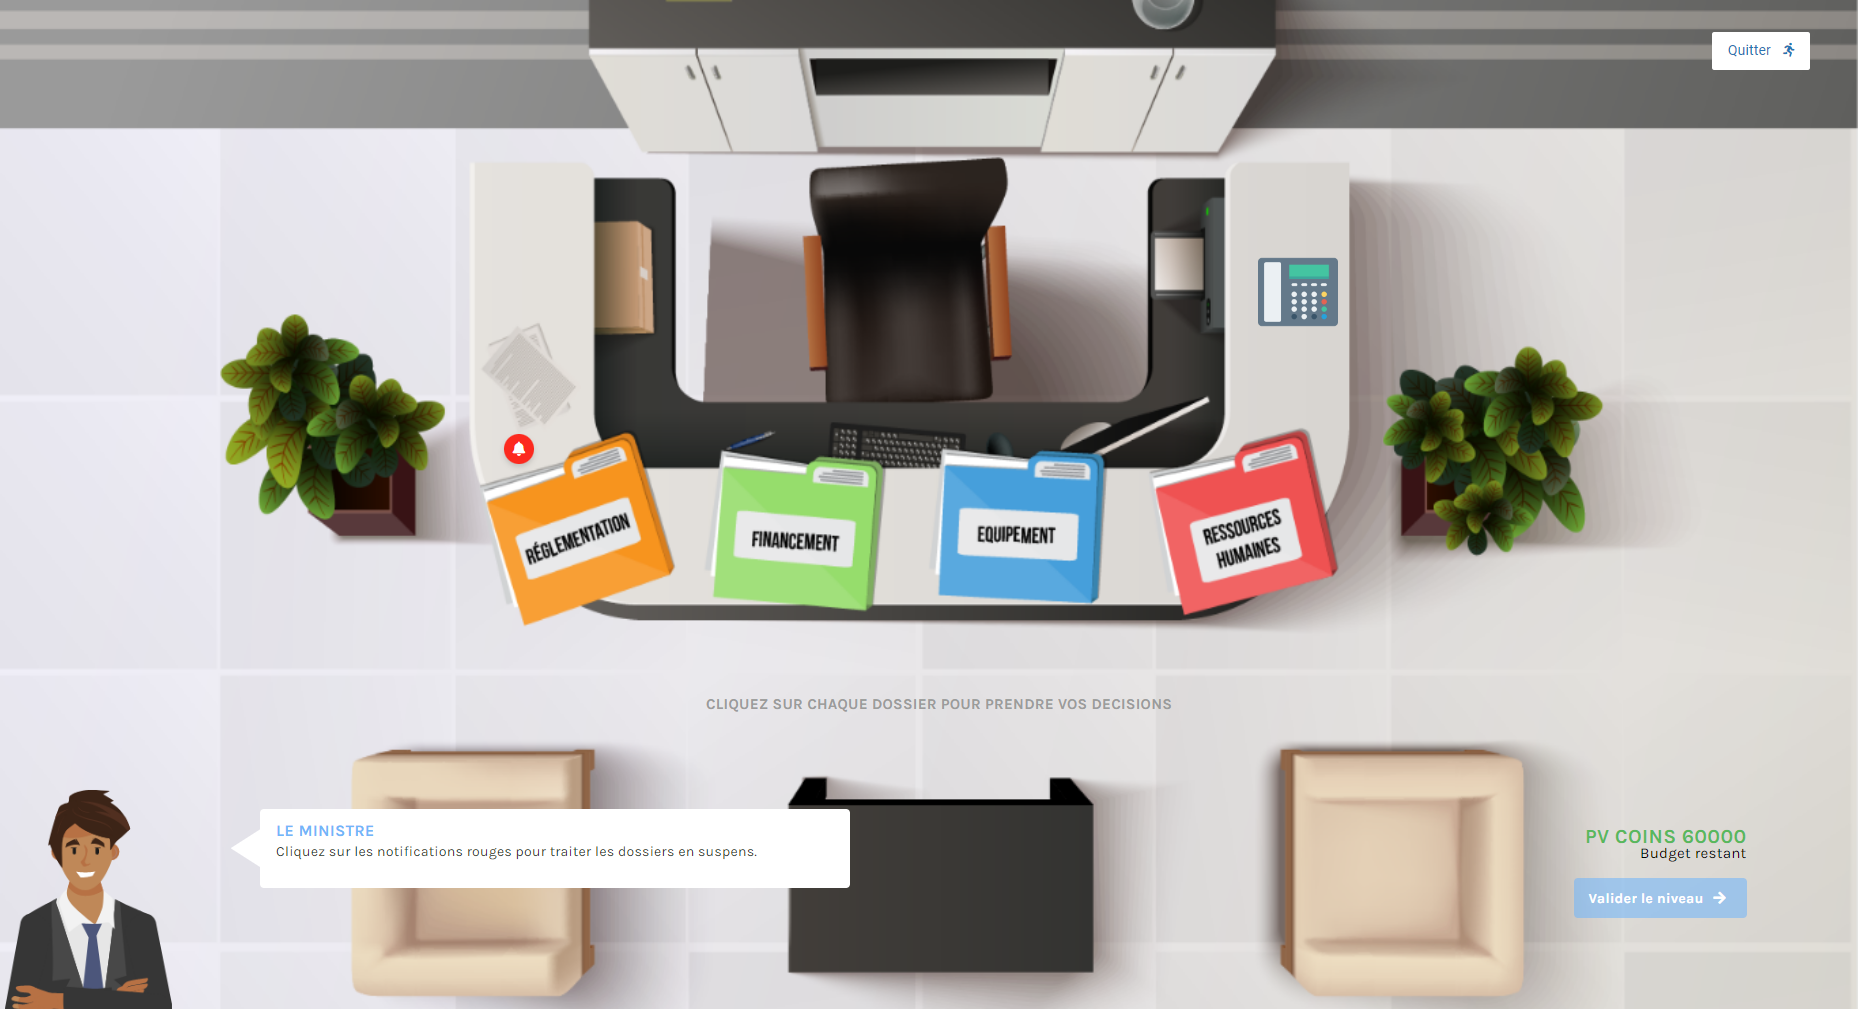
\includegraphics[scale=0.15]{images/1} 
\end{center} 




\begin{center}

\includegraphics[scale=0.15]{images/2} 
\end{center}


\begin{center}
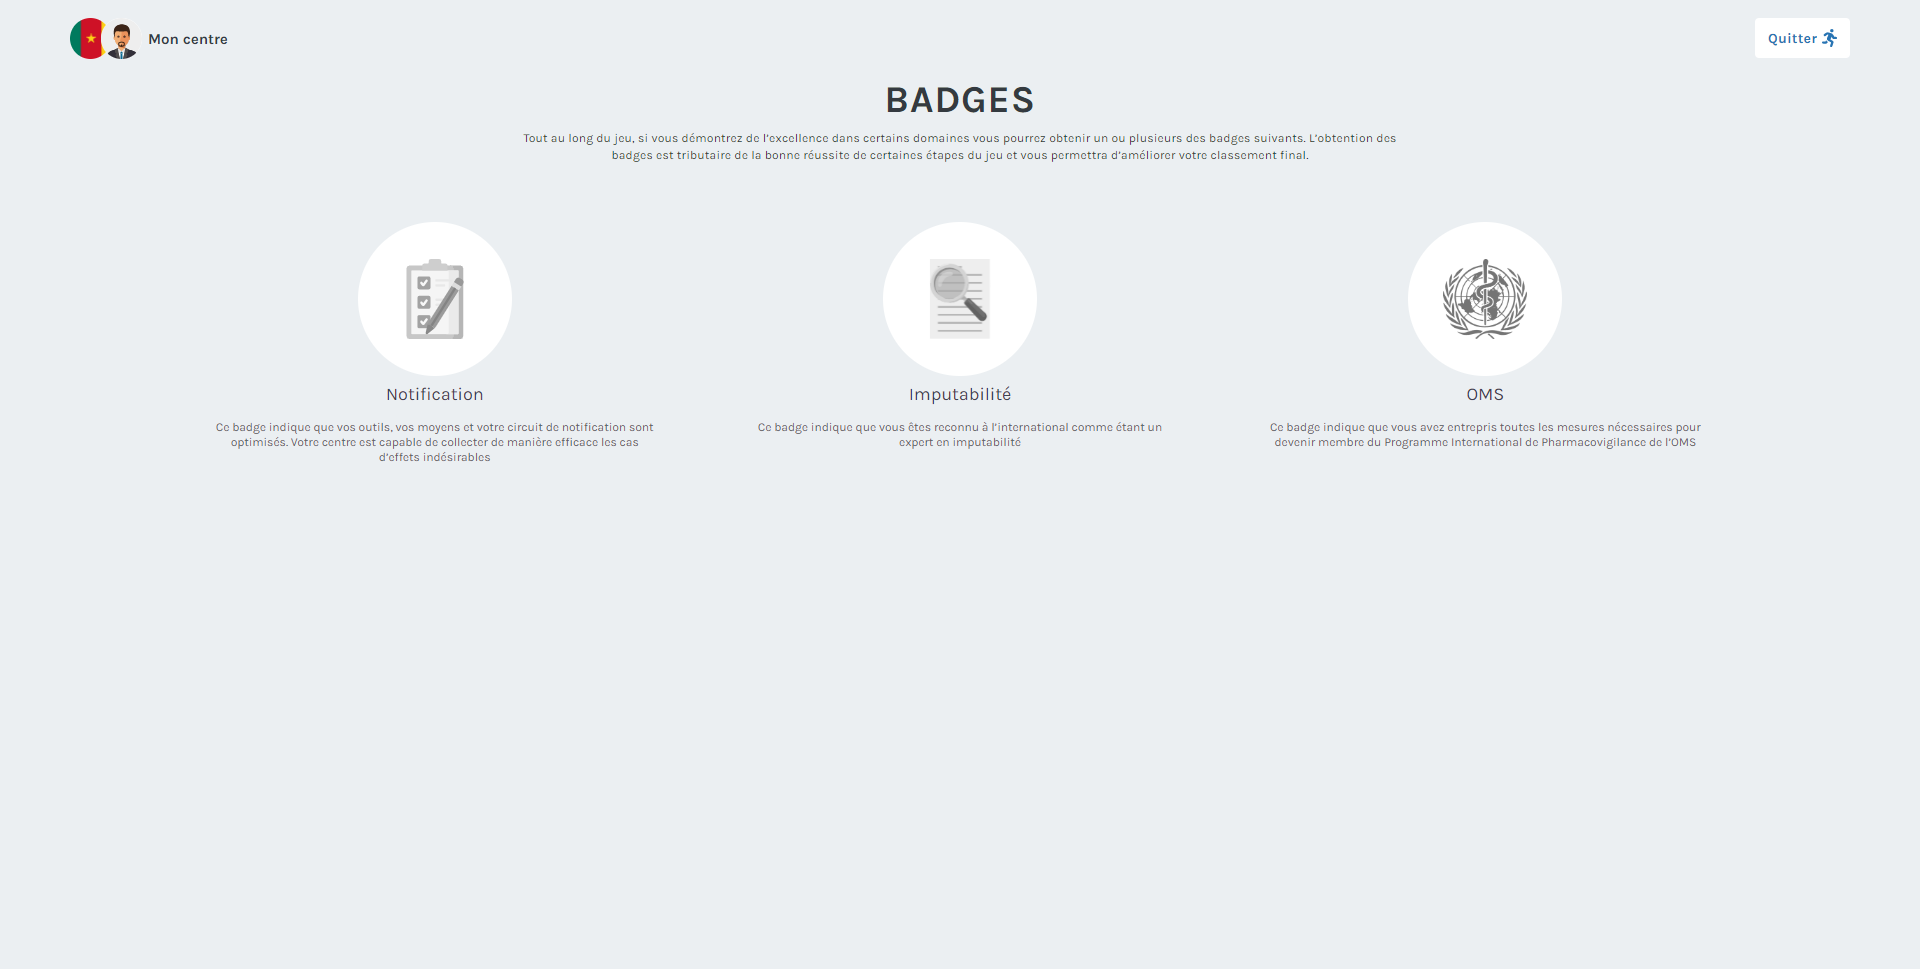
\includegraphics[scale=0.15]{images/5} 
\end{center}



\begin{center}
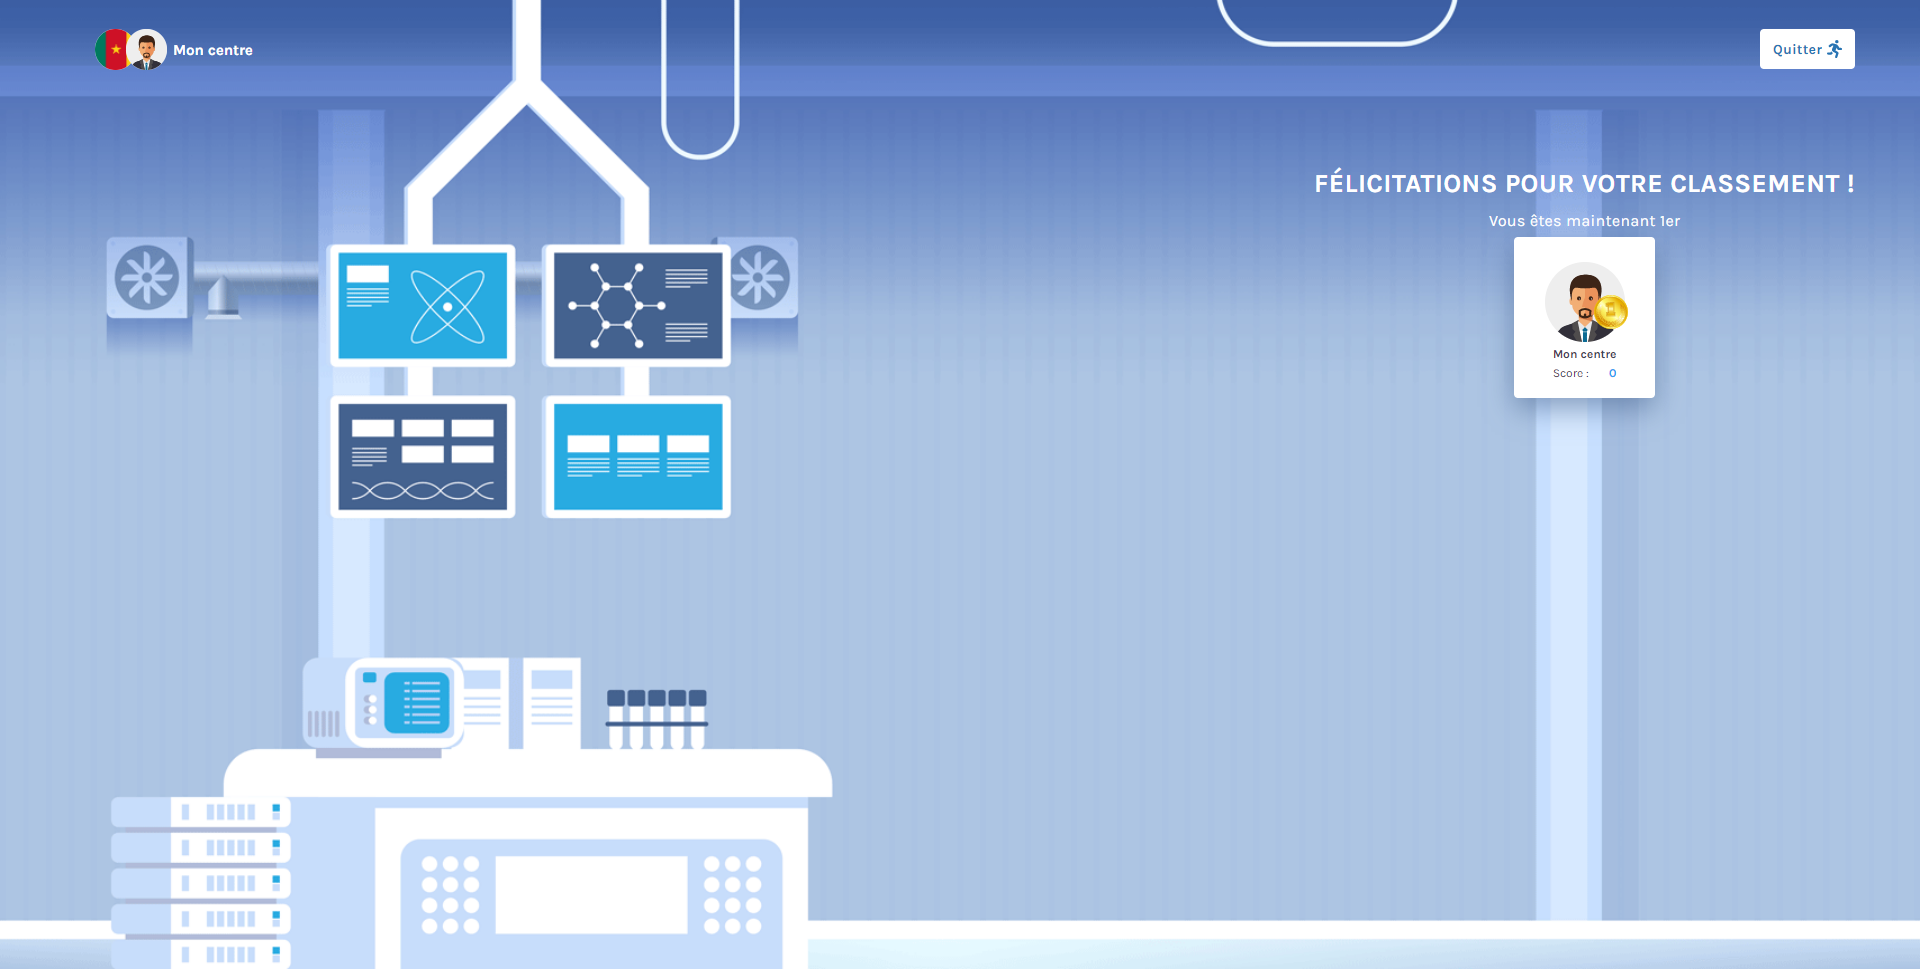
\includegraphics[scale=0.15]{images/4} 
\end{center}


\begin{center}
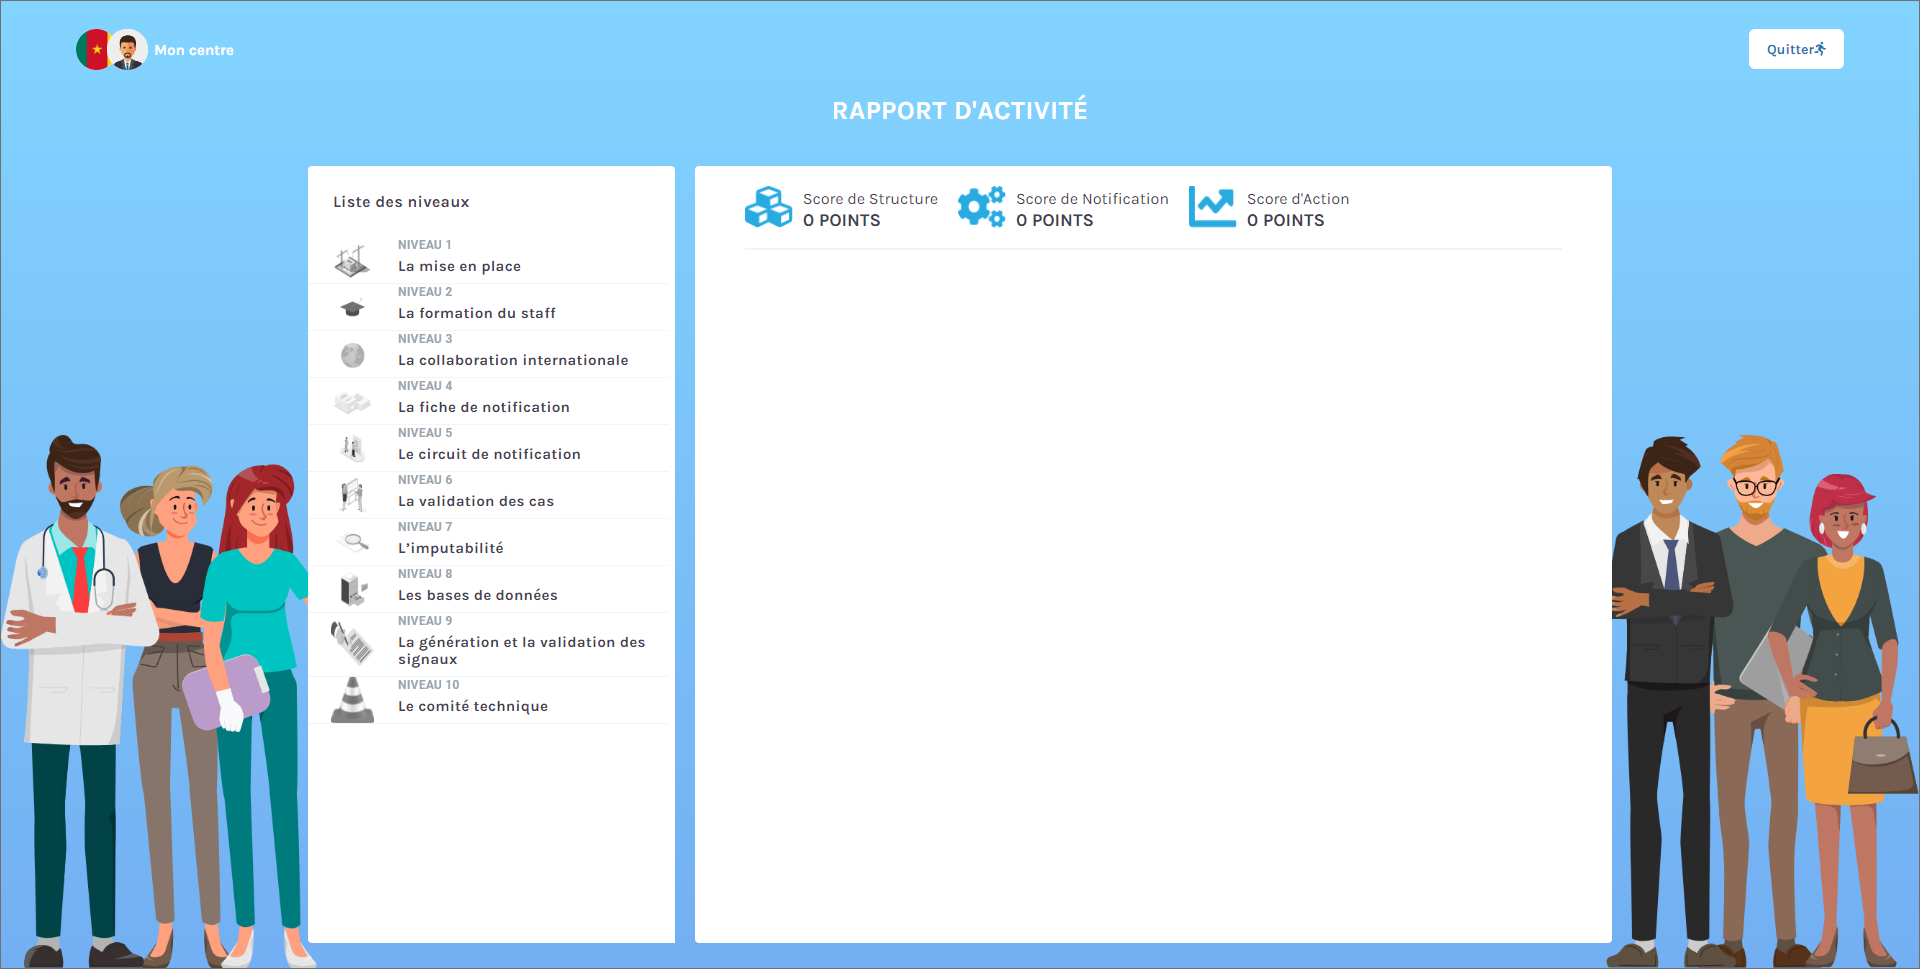
\includegraphics[scale=0.12]{images/3} 
\end{center}




\begin{center}

\includegraphics[scale=0.15]{images/6} 
\end{center}



\section{Conclusion}
La terminaison de cette étape marque la fin de notre projet, il reste à voir le résultat réél de ce projet et en tirer des conclusions, et puis voir des améliorations possible en guise de perspective.



\chapter*{Conclusion générale et perspectives}

Comme déjà montionné tout au long de ce rapport, le but de notre projet était de créer un système qui gère les données des patients en prenant en compte la dispertion des sources de ces données sur plusieurs bases de données qui représentent différents acteurs dans notre système de santé.

Nous avons en effet procéder à la conception et puis la réalisation de ce système en utilisant des outils qu'on utilise pour la première fois

En guise de perspectives, nous proposons que ce système comporte plus d'acteurs de santé avec des spécialités variés, et aussi la possibilité de travailler avec plusieurs base de données de différents fournisseurs (Oracle , Sql Server , Mongo DB ...) 

Enfin ce projet nous a offert l'opportunité de mettre en pratique nos connaissances théoriques sur un projet réel qui a poussé notre réflexion, et nous a incité à apprendre à travailler avec des nouvelles outils, ainsi à l'instar des autres projets faites à l'école nous avons consolidé notre abilité à travailler en groupe et de collaborer.



%\chapter*{Bibliographie}

ici c'est la bibliographie






%\input{./existant.tex}

 %\input{./besoins.tex}


%\input{./resultats.tex}



\newpage

%récupérer les citation avec "/footnotemark"
\nocite{*}

%choix du style de la biblio
\bibliographystyle{plain}
%inclusion de la biblio
\bibliography{bibliographie}
%voir wiki pour plus d'information sur la syntaxe des entrées d'une bibliographie
%\thispagestyle{empty}

\end{document}